\documentclass[aspectratio=169,12pt]{beamer}
\usepackage[utf8]{inputenc}
\usepackage{amsmath, amssymb}
\usepackage{booktabs}
\usepackage{colortbl}
\usepackage{hyperref}
\usepackage{makecell}
\usepackage{ragged2e}
\usepackage{bytefield}
\usepackage{tikz}
\usetikzlibrary{arrows.meta, positioning, shapes.geometric, calc, tikzmark, shapes.misc}
\usetheme{Madrid}

\title{Computer Structure}
\subtitle{Pipeline}
\author{Lihu Rappoport}
\date{}

\begin{document}

\frame{\titlepage}

\begin{frame}[t]{Five‑stage Pipeline}
\centering
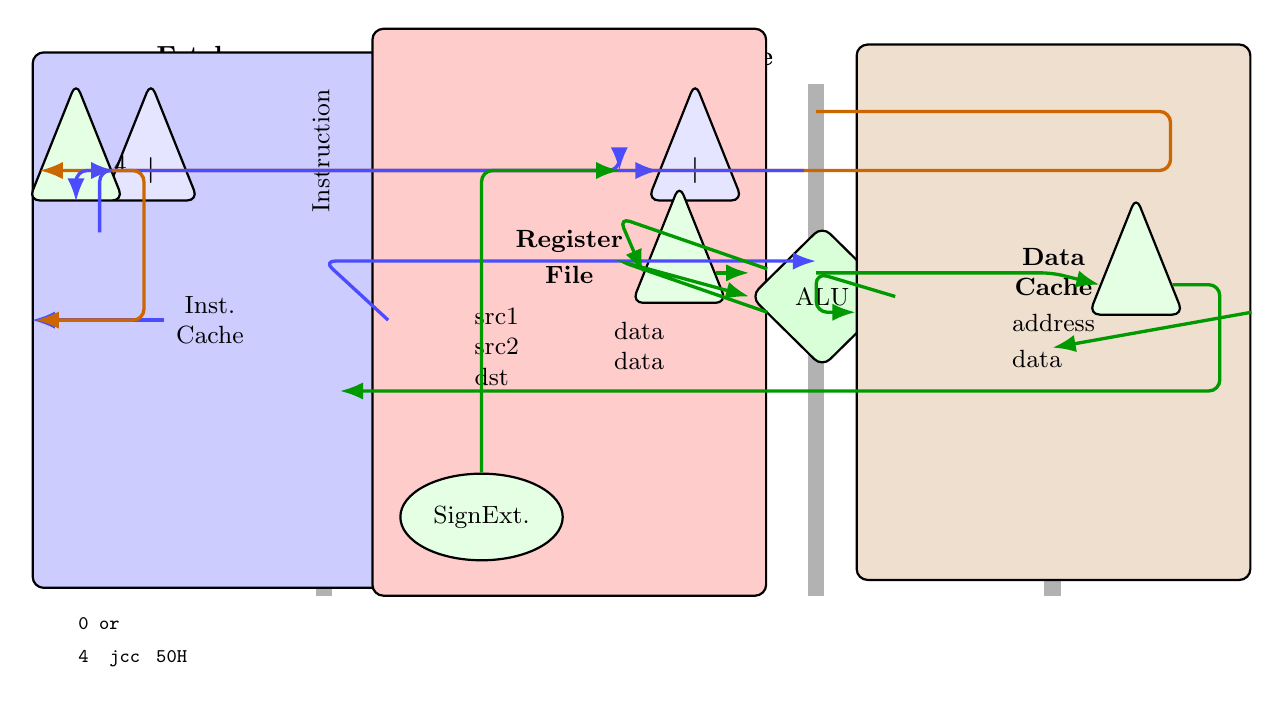
\begin{tikzpicture}[
    x=0.5cm, y=0.5cm,
    >=Latex,
    font=\small,
    rounded corners,
    thick,
    % Blocks
    block/.style={draw, rounded corners, align=center, thick},
    pc/.style    ={block, fill=blue!20, minimum width=1.6cm, minimum height=2.2cm},
    icache/.style={block, fill=blue!20, minimum width=4.5cm, minimum height=6.8cm},
    regfile/.style={block, fill=red!20,  minimum width=5.0cm, minimum height=7.2cm},
    dcache/.style={block, fill=brown!25, minimum width=5.0cm, minimum height=6.8cm},
    alu/.style   ={draw, diamond, aspect=2, minimum size=1.8cm, fill=green!15, thick},
    sign/.style  ={draw, ellipse, fill=green!10, minimum width=1.6cm, minimum height=1.1cm},
    mux/.style   ={draw, isosceles triangle, isosceles triangle stretches,
                   shape border rotate=90, minimum height=1.5cm, minimum width=1.2cm, fill=green!10},
    add/.style   ={draw, isosceles triangle, isosceles triangle stretches,
                   shape border rotate=90, minimum height=1.5cm, minimum width=1.2cm, fill=blue!10},
    % Pipes and wires
    pipe/.style  ={draw=black!30, line width=6pt},
    wireI/.style ={very thick, draw=blue!70,  ->},
    wireD/.style ={very thick, draw=green!60!black, ->},
    wirePC/.style={very thick, draw=orange!80!black, ->}
]

% Convenient x-positions for the pipeline registers
\def\pA{6.5}   % between Fetch and Decode
\def\pB{14}    % between Decode and Execute
\def\pC{19}    % between Execute and Memory
\def\pD{25}    % between Memory and WB

% Pipeline registers (vertical beige bars)
\draw[pipe] (\pA,-8.5) -- (\pA,4.5);
\draw[pipe] (\pB,-8.5) -- (\pB,4.5);
\draw[pipe] (\pC,-8.5) -- (\pC,4.5);
\draw[pipe] (\pD,-8.5) -- (\pD,4.5);

% Stage titles
\node[font=\bfseries] at ( 3.2,5.2) {Fetch};
\node[font=\bfseries] at (10.2,5.2) {Decode};
\node[font=\bfseries] at (16.5,5.2) {Execute};
\node[font=\bfseries] at (22.2,5.2) {Memory};
\node[font=\bfseries] at (27.8,5.2) {WB};

% --------------------------- Fetch -----------------------------------
\node[pc]    (pc) at (0.8,-1.5) {PC};
\node[icache](ic) at (3.6,-1.5) {Inst.\\Cache};

% PC+4 and next-PC mux
\node[add] (add4)  at (2.1,2.3) {};
\node       at (add4) {\Large $+$};
\node[anchor=west] at ($(add4)+(-1.2,0.15)$) {4};
\node[mux] (pcsel) at (0.2,2.3) {};

% -------------------------- Decode -----------------------------------
\node[regfile,anchor=west] (rf) at (\pA+1.2,-1.3) {%
\textbf{Register}\\[2pt]\textbf{File}\\[6pt]
\begin{tabular}{@{}l@{}}
src1\\
src2\\
dst
\end{tabular}\hspace{1.1cm}
\begin{tabular}{@{}l@{}}
data\\
data\\
\end{tabular}
};
\node[sign] (sext) at (10.5,-6.5) {Sign\\Ext.};

% -------------------------- Execute ----------------------------------
\node[add,anchor=west] (badd) at (\pB+1.0,2.3) {};
\node at (badd) {\Large $+$};
\node[mux,anchor=west] (amux) at (\pB+0.6,-0.3) {};
\node[alu,anchor=west] (alu) at (\pB+3.3,-0.9) {ALU};

% --------------------------- Memory ----------------------------------
\node[dcache,anchor=west] (dc) at (\pC+1.0,-1.3) {%
\textbf{Data}\\\textbf{Cache}\\[4pt]
\begin{tabular}{@{}l@{}}
address\\[2pt]
data
\end{tabular}
};

% --------------------------- Writeback -------------------------------
\node[mux,anchor=west] (wbmux) at (\pD+1.2,-0.6) {};

% Label on first pipe
\node[rotate=90,anchor=south] at (\pA+0.4,2.8) {Instruction};

% ======================== Wiring =====================================

% Blue: instruction path
\draw[wireI] (pc.east) -- (ic.west);
\draw[wireI] (ic.east) -- (\pA,0.0) -- (\pB,0.0) -- (\pC,0.0);
\draw[wireI] (pc.north) |- (add4.west);
\draw[wireI] (add4.east) -| (\pB,2.3);
\draw[wireI] (\pB,2.3) -- (badd.west);

% Orange: long next‑PC/bypass control (for illustration)
\draw[wirePC] (\pC,3.8) -- (\pD,3.8) -- ++(3.0,0) |- (pcsel.west);

% Close the PC update loop
\draw[wireI] (badd.east) -- ++(2.0,0) -| (pcsel.south);
\draw[wirePC] (pcsel.east) -- ++(0.8,0) |- (pc.west);

% Green: data path
\coordinate (rfout1) at ($(rf.east)+(0,1.1)$);
\coordinate (rfout2) at ($(rf.east)+(0,0.0)$);

\draw[wireD] (rfout1) -- (\pB,1.1) -- (amux.west);      % src1 -> mux
\draw[wireD] (rfout2) -- (\pB,0.0) -- (alu.west);        % src2 -> ALU
\draw[wireD] (amux.east) -- (alu.west |- amux.east);     % mux -> ALU

\draw[wireD] (sext.north) |- (\pB,2.3);                  % sign-ext to branch adder

\draw[wireD] (alu.east) -- (\pC,-0.3) |- (dc.west);      % ALU addr -> D$ 
\draw[wireD] (dc.east) -- (\pD,-2.2);                    % D$ data -> WB pipe
\draw[wireD] (\pC,-0.3) -- (\pD,-0.3) -- (wbmux.west);   % ALU result -> WB mux
\draw[wireD] (wbmux.east) -- ++(1.2,0) |- ($(rf.west)+(-0.8,-2.0)$); % write-back to RF

% Small legend text from the original picture (optional)
\node[anchor=west,font=\ttfamily\scriptsize] at (0,-9.2) {0 or};
\node[anchor=west,font=\ttfamily\scriptsize] at (0,-10.1) {4\quad jcc\; 50H};

\end{tikzpicture}
\end{frame}


%% Slide: A Basic Processor
\begin{frame}{A Basic Processor}
    \centering
    \begin{tikzpicture}[scale=0.8]
        % Placeholder for processor diagram
        \node[draw, rectangle, minimum width=12cm, minimum height=6cm, dashed, align=center] {
            \Large Processor Pipeline Diagram\\
            \normalsize (Fetch $\rightarrow$ Decode $\rightarrow$ Execute $\rightarrow$ Memory $\rightarrow$ Write Back)
        };
    \end{tikzpicture}
\end{frame}

%% Slide: Pipelined Car Assembly
\begin{frame}{Pipelined Car Assembly}
    \centering
    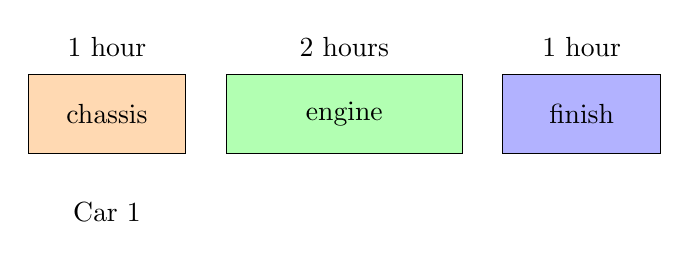
\begin{tikzpicture}[scale=0.9]
        \node[draw, fill=orange!30, minimum width=2cm, minimum height=1cm] (chassis) {chassis};
        \node[draw, fill=green!30, minimum width=3cm, minimum height=1cm, right=0.5cm of chassis] (engine) {engine};
        \node[draw, fill=blue!30, minimum width=2cm, minimum height=1cm, right=0.5cm of engine] (finish) {finish};
        
        \node[above=0.1cm of chassis] {1 hour};
        \node[above=0.1cm of engine] {2 hours};
        \node[above=0.1cm of finish] {1 hour};
        
        \node[below=0.5cm of chassis] {Car 1};
    \end{tikzpicture}
    
    \vspace{1cm}
    Time: 00:00
\end{frame}

%% Slide: Pipelined Car Assembly - Multiple Cars
\begin{frame}{Pipelined Car Assembly}
    \begin{itemize}
        \item Car 2 waited an hour after finishing station 1 for Car 1 to finish station 2
        \item Pipeline latency is 5 hours
        \item Pipeline throughput is one car every 2 hours
    \end{itemize}
    
    \centering
    
\begin{tikzpicture}[scale=0.8]
        % Simplified pipeline representation
        \node[draw, dashed, minimum width=10cm, minimum height=2cm] {
            Pipeline stages with multiple cars
        };
    \end{tikzpicture}
\end{frame}

%% Slide: Pipelining Instructions
\begin{frame}{Pipelining Instructions}
    \begin{columns}
        \column{0.5\textwidth}
        \textbf{Sequential Execution:}
        \begin{itemize}
            \item 8 ns per instruction
            \item Total: 24 ns for 3 instructions
        \end{itemize}
        
        \column{0.5\textwidth}
        \textbf{Pipelined Execution:}
        \begin{itemize}
            \item 2 ns per stage
            \item Total: 14 ns for 3 instructions
        \end{itemize}
    \end{columns}
    
    \vspace{0.5cm}
    \centering
    Program execution order:
    \begin{enumerate}
        \item \texttt{lw R1, 100(R0)}
        \item \texttt{lw R2, 200(R0)}
        \item \texttt{lw R3, 300(R0)}
    \end{enumerate}
    
    \textbf{Ideal speedup = Number of pipeline stages}
\end{frame}

%% Slide: Pipelining
\begin{frame}{Pipelining}
    \begin{itemize}
        \item Pipelining does not reduce the \textcolor{red}{latency} of single task, it increases the \textcolor{green}{throughput} of entire workload
        \item Potential speedup = Number of pipe stages
        \begin{itemize}
            \item Pipeline rate is limited by the slowest pipeline stage
            \item[$\Rightarrow$] Partition the pipe to many pipe stages
            \item[$\Rightarrow$] Make the longest pipe stage to be as short as possible
            \item[$\Rightarrow$] Balance the work in the pipe stages
        \end{itemize}
        \item Pipeline adds overhead (e.g., latches)
        \begin{itemize}
            \item Time to "fill" pipeline and time to "drain" it reduces speedup
            \item Stall for dependencies
            \item[$\Rightarrow$] Too many pipe-stages start to lose performance
        \end{itemize}
        \item IPC of an ideal pipelined machine is 1
        \begin{itemize}
            \item Every clock one instruction finishes
        \end{itemize}
    \end{itemize}
\end{frame}

%% Slide: Pipelined CPU
\begin{frame}{Pipelined CPU}
    \centering
    \begin{tikzpicture}[scale=0.7]
        % Placeholder for pipelined CPU diagram
        \node[draw, rectangle, minimum width=14cm, minimum height=7cm, dashed, align=center] {
            \Large Pipelined CPU Architecture\\
            \normalsize (Fetch $\rightarrow$ Decode $\rightarrow$ Execute $\rightarrow$ Memory $\rightarrow$ WB)\\
            \small with pipeline latches between stages
        };
    \end{tikzpicture}
\end{frame}

%% Slide: Structural Hazard
\begin{frame}{Structural Hazard}
    \begin{itemize}
        \item Different instructions using the same resource at the same time
        \item \textbf{Register File:}
        \begin{itemize}
            \item Accessed in 2 stages:
            \begin{itemize}
                \item Read during stage 2 (ID)
                \item Write during stage 5 (WB)
            \end{itemize}
            \item Solution: 2 read ports, 1 write port
        \end{itemize}
        \item \textbf{Memory:}
        \begin{itemize}
            \item Accessed in 2 stages:
            \begin{itemize}
                \item Instruction Fetch during stage 1 (IF)
                \item Data read/write during stage 4 (MEM)
            \end{itemize}
            \item Solution: separate instruction cache and data cache
        \end{itemize}
        \item Each functional unit can only be used \textcolor{green}{once} per instruction
        \item Each functional unit must be used at the \textcolor{green}{same} stage for all instructions
    \end{itemize}
\end{frame}

%% Slide: Pipeline Example
\begin{frame}{Pipeline Example: cycle 1}
    \begin{columns}
        \column{0.4\textwidth}
        \begin{tabular}{ll}
            0 & \texttt{lw R10,9(R1)}\\
            4 & \texttt{sub R11,R2,R3}\\
            8 & \texttt{and R12,R4,R5}\\
            12 & \texttt{or R13,R6,R7}
        \end{tabular}
        
        \column{0.6\textwidth}
        \centering
        PC = 0
        \vspace{0.5cm}
        
        \begin{tikzpicture}[scale=0.6]
            \node[draw, dashed, minimum width=8cm, minimum height=3cm, align=center] {
                Pipeline State Diagram\\
                (Cycle 1)
            };
        \end{tikzpicture}
    \end{columns}
\end{frame}

%% Slide: RAW Dependency
\begin{frame}{RAW Dependency}
    \begin{columns}
        \column{0.5\textwidth}
        Program execution order:
        \begin{enumerate}
            \item \texttt{sub R2, R1, R3}
            \item \texttt{and R12, \textcolor{red}{R2}, R5}
            \item \texttt{or R13, R6, \textcolor{red}{R2}}
            \item \texttt{add R14, \textcolor{red}{R2}, \textcolor{red}{R2}}
            \item \texttt{sw R15, 100(\textcolor{red}{R2})}
        \end{enumerate}
        
        \column{0.5\textwidth}
        \centering
        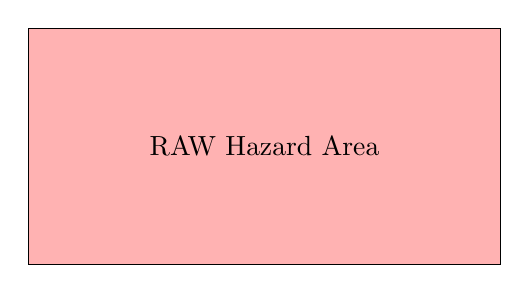
\begin{tikzpicture}[scale=0.5]
            % Pipeline stages showing dependency
            \node[draw, fill=red!30, minimum width=6cm, minimum height=3cm] {
                RAW Hazard Area
            };
        \end{tikzpicture}
    \end{columns}
\end{frame}

%% Slide: Using Bypass to Solve RAW Dependency
\begin{frame}{Using Bypass to Solve RAW Dependency}
    \begin{itemize}
        \item Bypass result directly from EXE output to EXE input
        \item No stall needed when bypass is possible
        \item Hardware forwards data from:
        \begin{itemize}
            \item EXE/MEM pipeline register
            \item MEM/WB pipeline register
        \end{itemize}
    \end{itemize}
    
    \centering
    \begin{tikzpicture}[scale=0.7]
        \node[draw, dashed, minimum width=10cm, minimum height=4cm] {
            Bypass/Forwarding Hardware Diagram
        };
    \end{tikzpicture}
\end{frame}

%% Slide: Bypass Control
\begin{frame}[fragile]{Bypass Control}
    \textbf{L3\_reg\_wr = L3.RegWrite and (L3.opcode != lw)}
    
    \vspace{0.3cm}
    \textbf{Forwarding from EXE (L3):}
    \begin{itemize}
        \item \small if (L3\_reg\_wr and (L3.dst == L2.src1)) ALUSelA = 1
        \item \small if (L3\_reg\_wr and (L3.dst == L2.src2)) ALUSelB = 1
    \end{itemize}
    
    \vspace{0.3cm}
    \textbf{Forwarding from MEM (L4):}
    \begin{itemize}
        \item \small if (L4.RegWrite and ((not L3\_reg\_wr) or (L3.dst $\neq$ L2.src1))\\
              and (L4.dst = L2.src1)) ALUSelA = 2
        \item \small if (L4.RegWrite and ((not L3\_reg\_wr) or (L3.dst $\neq$ L2.src2))\\
              and (L4.dst = L2.src2)) ALUSelB = 2
    \end{itemize}
\end{frame}

%% Slide: Register File Split
\begin{frame}{Register File Split}
    \begin{itemize}
        \item Register file is written during first half of the cycle
        \item Register file is read during second half of the cycle
        \item[$\Rightarrow$] Register file is written before it is read $\Rightarrow$ returns the correct data
    \end{itemize}
    
    \centering
    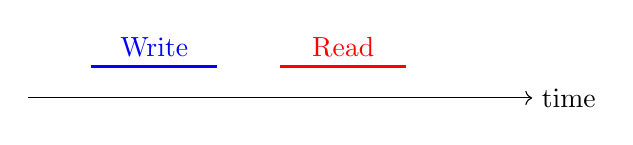
\begin{tikzpicture}[scale=0.8]
        % Timeline showing register file operations
        \draw[->] (0,0) -- (8,0) node[right] {time};
        \draw[thick, blue] (1,0.5) -- (3,0.5) node[midway, above] {Write};
        \draw[thick, red] (4,0.5) -- (6,0.5) node[midway, above] {Read};
    \end{tikzpicture}
\end{frame}

%% Slide: Can't Always Bypass
\begin{frame}{Can't Always Bypass}
    \begin{itemize}
        \item Load word can still cause a hazard
        \begin{itemize}
            \item An instruction tries to read a register following a load instruction that writes to the same register
        \end{itemize}
        \item A hazard detection unit is needed to "stall" the load instruction
    \end{itemize}
    
    Program execution order:
    \begin{enumerate}
        \item \texttt{lw \textcolor{red}{R2}, 30(R1)}
        \item \texttt{and R12, \textcolor{red}{R2}, R5}
        \item \texttt{or R13, R6, \textcolor{red}{R2}}
        \item \texttt{add R14, \textcolor{red}{R2}, \textcolor{red}{R2}}
        \item \texttt{sw R15, 100(\textcolor{red}{R2})}
    \end{enumerate}
\end{frame}

%% Slide: Stall If Cannot Bypass
\begin{frame}[fragile]{Stall If Cannot Bypass}
    \begin{verbatim}
if (L2.RegWrite and (L2.opcode == lw) and 
    ((L2.dst == L1.src1) or (L2.dst == L1.src2))) 
then stall
    \end{verbatim}
    
    \vspace{0.5cm}
    \begin{itemize}
        \item De-assert the enable to the L1 latch, and to the IP
        \begin{itemize}
            \item The dependent instruction (and) stays another cycle in L1
        \end{itemize}
        \item Issue a NOP into the L2 latch (instead of the stalled inst.)
        \item Allow the stalling instruction (lw) to move on
    \end{itemize}
    
    \centering
    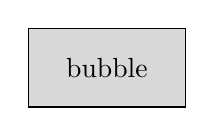
\begin{tikzpicture}[scale=0.6]
        \node[draw, fill=gray!30, minimum width=2cm, minimum height=1cm] {bubble};
    \end{tikzpicture}
\end{frame}

%% Slide: Software Scheduling to Avoid Load Hazards
\begin{frame}[fragile]{Software Scheduling to Avoid Load Hazards}
    Example: code for (assume all variables are in memory):
    \begin{center}
        \texttt{a = b + c;}\\
        \texttt{d = e - f;}
    \end{center}
    
    \begin{columns}
        \column{0.5\textwidth}
        \textbf{Slow code:}
        \begin{verbatim}
LW   Rb,b
LW   Rc,c
Stall
ADD  Ra,Rb,Rc
SW   a,Ra
LW   Re,e
LW   Rf,f
Stall
SUB  Rd,Re,Rf
SW   d,Rd
        \end{verbatim}
        
        \column{0.5\textwidth}
        \textbf{Fast code:}
        \begin{verbatim}
LW   Rb,b
LW   Rc,c
LW   Re,e
ADD  Ra,Rb,Rc
LW   Rf,f
SW   a,Ra
SUB  Rd,Re,Rf
SW   d,Rd
        \end{verbatim}
    \end{columns}
    
    \vspace{0.5cm}
    \centering
    \textit{Instruction order can be changed as long as the correctness is kept}
\end{frame}

%% Section: Control Hazards
\begin{frame}
    \begin{center}
        \Huge Control Hazards
    \end{center}
\end{frame}

%% Slide: Control Hazard on Branches
\begin{frame}[fragile]{Control Hazard on Branches}
    \texttt{jcc target; if cond then PC $\leftarrow$ target}
    
    \begin{itemize}
        \item The target is saved in the instruction relative to the address of the fall-through instruction
        \item Most conditional jumps are short (if and loop) $\Rightarrow$ save bits in the instruction encoding
        \item The 3 instructions following the branch get into the pipe even if the branch is taken
    \end{itemize}
    
    \begin{columns}
        \column{0.4\textwidth}
        \begin{verbatim}
0  or
4  jcc 50H
8  and
12 sw
16 sub
        \end{verbatim}
        
        \column{0.6\textwidth}
        \centering
        \begin{tikzpicture}[scale=0.6]
            \node[draw, dashed, minimum width=6cm, minimum height=3cm] {
                Branch Pipeline Diagram
            };
        \end{tikzpicture}
    \end{columns}
\end{frame}

%% Slide: Control Hazard: Stall
\begin{frame}{Control Hazard: Stall}
    \begin{itemize}
        \item Stall pipe when branch is encountered until resolved
        \item Stall impact: assumptions
        \begin{itemize}
            \item CPI = 1
            \item 20\% of instructions are branches
            \item Stall 3 cycles on every branch
            \item[$\Rightarrow$] CPI\textsubscript{new} = 1 + 0.2 × 3 = 1.6
        \end{itemize}
    \end{itemize}
    
    \vspace{0.5cm}
    \centering
    (CPI\textsubscript{new} = CPI\textsubscript{Ideal} + avg. stall cycles / instr.)
    
    \vspace{0.5cm}
    \textbf{We lose 60\% of the performance}
\end{frame}

%% Slide: Control Hazard: Predict Not Taken
\begin{frame}{Control Hazard: Predict Not Taken}
    \begin{itemize}
        \item Execute instructions from the fall-through (not-taken) path
        \begin{itemize}
            \item As if there is no branch
            \item If the branch is not-taken (~50\%), no penalty is paid
        \end{itemize}
        \item If branch actually taken
        \begin{itemize}
            \item Flush the fall-through path instructions before they change the machine state (memory / registers)
            \item Fetch the instructions from the correct (taken) path
        \end{itemize}
        \item Assuming 20\% of instructions are branches and ~50\% branches not taken on average
        \begin{itemize}
            \item CPI\textsubscript{new} = 1 + (0.2 × 0.5) × 3 = 1.3
        \end{itemize}
    \end{itemize}
\end{frame}

%% Slide: Dynamic Branch Prediction
\begin{frame}{Dynamic Branch Prediction}
    \begin{itemize}
        \item Add a \textbf{Branch Target Buffer (BTB)} that predicts (at fetch)
        \begin{itemize}
            \item Instruction is a branch
            \item Branch taken / not-taken
            \item Taken branch target
        \end{itemize}
        \item BTB allocated at execute – after all branch info is known
        \item BTB is looked up at instruction fetch
    \end{itemize}
    
    \centering
    \begin{tabular}{|c|c|c|}
        \hline
        Branch IP & Target IP & History\\
        \hline
        & & \\
        & & \\
        \hline
    \end{tabular}
    
    \vspace{0.5cm}
    BTB Structure
\end{frame}

%% Slide: BTB
\begin{frame}{BTB}
    \begin{itemize}
        \item \textbf{Allocation} – at Decode / EXE
        \begin{itemize}
            \item Allocate instructions identified as branches (after decode)
            \item Not taken branches need not be allocated
            \item BTB miss implicitly predicts not-taken
        \end{itemize}
        \item \textbf{Prediction} – at Fetch
        \begin{itemize}
            \item BTB lookup is done parallel to IC lookup
            \item BTB provides:
            \begin{itemize}
                \item Indication that the instruction is a branch (BTB hits)
                \item Branch predicted target
                \item Branch predicted direction
                \item Branch predicted type (e.g., conditional, unconditional)
            \end{itemize}
        \end{itemize}
        \item \textbf{Update} (when branch outcome is known – at EXE)
        \begin{itemize}
            \item Branch target
            \item Branch history (taken / not-taken)
        \end{itemize}
    \end{itemize}
\end{frame}

%% Slide: BTB (cont.)
\begin{frame}{BTB (cont.)}
    \begin{itemize}
        \item \textbf{Wrong prediction}
        \begin{itemize}
            \item Predict not-taken, actual taken
            \item Predict taken, actual not-taken, or actual taken but wrong target
        \end{itemize}
        \item \textbf{In case of wrong prediction – flush the pipeline}
        \begin{itemize}
            \item Reset latches (same as making all instructions to be NOPs)
            \item Select the PC source to be from the correct path
            \item Need get the fall-through with the branch
            \item Start fetching instruction from correct path
        \end{itemize}
        \item \textbf{Assuming P\% correct prediction rate}
        \begin{itemize}
            \item CPI\textsubscript{new} = 1 + (0.2 × (1-P)) × 3
            \item For example, if P=0.7
            \item CPI\textsubscript{new} = 1 + (0.2 × 0.3) × 3 = 1.18
        \end{itemize}
    \end{itemize}
\end{frame}

%% Slide: Adding a BTB to the Pipeline
\begin{frame}{Adding a BTB to the Pipeline}
    \centering
    \begin{tikzpicture}[scale=0.7]
        % Placeholder for BTB pipeline integration diagram
        \node[draw, rectangle, minimum width=14cm, minimum height=7cm, dashed, align=center] {
            \Large BTB Integration with Pipeline\\
            \normalsize BTB lookup parallel with I-cache lookup\\
            \small Predicted target and direction available at Fetch
        };
    \end{tikzpicture}
\end{frame}

%% Slide: Using The BTB
\begin{frame}{Using The BTB}
    \centering
    \begin{tikzpicture}[scale=0.8, node distance=1.5cm]
        % Flowchart for BTB usage
        \node[draw, rectangle] (pc) {PC moves to next instruction};
        \node[draw, rectangle, below left=of pc, align=center] (imem) {Inst Mem gets PC\\and fetches new inst};
        \node[draw, rectangle, below right=of pc, align=center] (btb) {BTB gets PC\\and looks it up};
        \node[draw, diamond, below=of btb] (hit) {BTB Hit?};
        \node[draw, diamond, below left=of hit] (taken) {Br taken?};
        \node[draw, rectangle, below=of taken] (pred) {PC $\leftarrow$ pred addr};
        \node[draw, rectangle, below right=of hit] (inc) {PC $\leftarrow$ PC + 4};
        
        \draw[->] (pc) -- (imem);
        \draw[->] (pc) -- (btb);
        \draw[->] (btb) -- (hit);
        \draw[->] (hit) -- node[left] {yes} (taken);
        \draw[->] (hit) -- node[right] {no} (inc);
        \draw[->] (taken) -- node[left] {yes} (pred);
        \draw[->] (taken) -- node[right] {no} (inc);
    \end{tikzpicture}
\end{frame}

%% Slide: Using The BTB (cont.)
\begin{frame}{Using The BTB (cont.)}
    \centering
    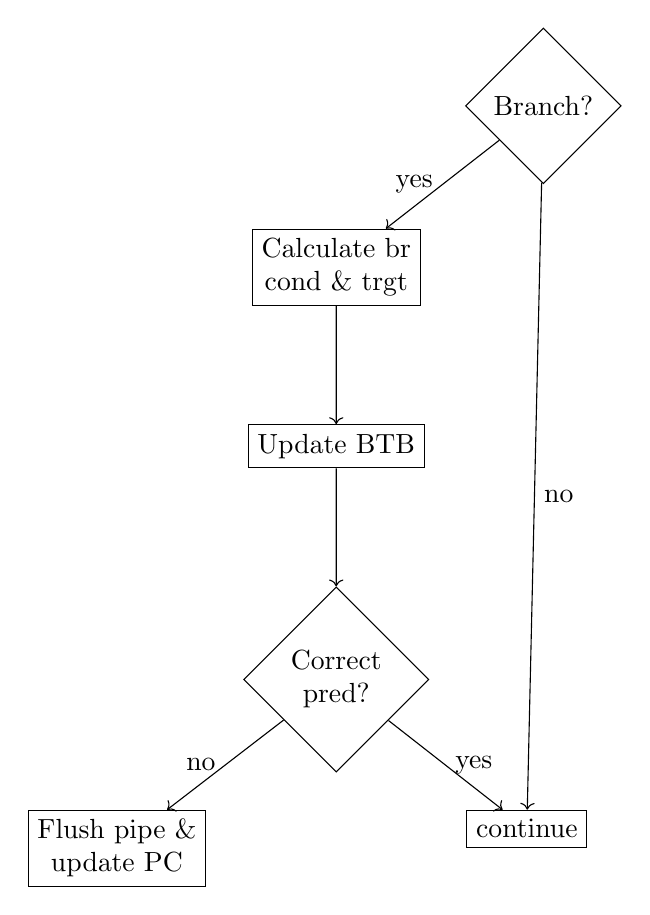
\begin{tikzpicture}[scale=0.8, node distance=1.5cm]
        % Continuation of BTB flowchart
        \node[draw, diamond] (branch) {Branch?};
        \node[draw, rectangle, below left=of branch, align=center] (calc) {Calculate br\\cond \& trgt};
        \node[draw, rectangle, below=of calc] (update) {Update BTB};
        \node[draw, diamond, below=of update, align=center] (correct) {Correct\\pred?};
        \node[draw, rectangle, below left=of correct, align=center] (flush) {Flush pipe \&\\update PC};
        \node[draw, rectangle, below right=of correct] (continue) {continue};
        
        \draw[->] (branch) -- node[left] {yes} (calc);
        \draw[->] (branch) -- node[right] {no} (continue);
        \draw[->] (calc) -- (update);
        \draw[->] (update) -- (correct);
        \draw[->] (correct) -- node[left] {no} (flush);
        \draw[->] (correct) -- node[right] {yes} (continue);
    \end{tikzpicture}
\end{frame}

\end{document}